\chapter{Empurrando Juntos} \label{cap:empurrandojuntos}

A observação do viés nas discussões nas redes sociais e em outras plataformas de interação social despertou o interesse
para a criação de novos sistemas capazes de contornar essa situação da polarização das mensagens trocadas.
Nesse sentido, surge o ``Empurrando Juntos'' como a ideia de uma plataforma online capaz 
de dar voz para a minoria e tornar as discussões mais efetivas para o propósito. Possibilitando ao usuário
identificar grupos de opinião e tendências em uma conversa \cite{empurrandojuntos}. 

Essa participação 
acontece de duas formas: comentando uma conversa ou votando em um comentário de outro participante. Entende-se por voto
o ato de concordar com o comentário realizado (uma espécie de \textit{like}) ou discordar do comentário. Além disso, é permitido
que o usuário pule aquele comentário, ou seja, não atribua nenhum tipo de voto \cite{empurrandojuntos}. 

Com os votos realizados, é possível agrupar pessoas que responderam de maneira parecida, ou seja, concordaram e
discordaram dos mesmos comentários. Com os grupos formados, é possível ver a convergência e divergência de opiniões, 
prover ao usuário uma visão ampliada acerca do assunto e promover a interação entre os usuários com 
pensamentos divergentes. A Figura \ref{fig:resumo_ej} ilustra o funcionamento completo do sistema.

\begin{figure}[h!]
\centering
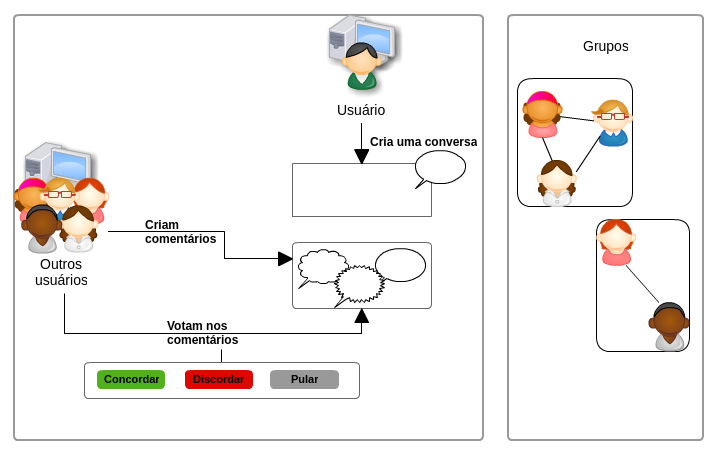
\includegraphics[scale=0.6]{figuras/resumo_ej.png}
\caption{Funcionamento do ``Empurrando Juntos''}
\label{fig:resumo_ej}
\end{figure}


